\documentclass[10pt,twocolumn,letterpaper]{article}
\usepackage[review]{cvpr}
\usepackage{array}
\usepackage{microtype}
\definecolor{cvprblue}{rgb}{0.21,0.49,0.74}
\usepackage[pagebackref,breaklinks,colorlinks,allcolors=cvprblue]{hyperref}
\usepackage[capitalize]{cleveref}
\def\confName{CVPR}
\def\confYear{2027}
\title{Beyond Spread: Diagnosing and Repairing Gaps in Generative Distributions}
\author{}
\hypersetup{pdftitle={Beyond Spread: Diagnosing and Repairing Gaps in Generative Distributions},pdfauthor={}}
\raggedbottom
\setlength{\hfuzz}{0.5pt}
\begin{document}
\maketitle
\begin{abstract}
A fast image generator can match overall variation while losing an entire
region of the image distribution. We introduce an audit that fixes a
reference, measures changes in regional probability and within-region
variation, and tests whether targeted interventions improve the intended
outcome on fresh samples. A finite-sample bound certifies when a regional loss
exceeds a declared magnitude. On a fixed natural-image model,
changing the covariance of the starting noise lowers a feature-based
distribution discrepancy by 32\% at two denoising calls per image and
raises coverage of real-image feature neighborhoods from 20.6\% to 28.8\%.
In a handwritten-digit experiment, ordinary training corrects a digit
overshoot at the same update budget, reducing mean digit-frequency error
by 59\% across three training seeds. Including images rejected by the
digit classifiers, the discrepancy across the full set of outcomes falls
by 42\%. In text-to-image generation, the same audit explains how pooled
variation can fall while variation within individual prompts rises.
\end{abstract}

\begin{figure*}[t]
\centering
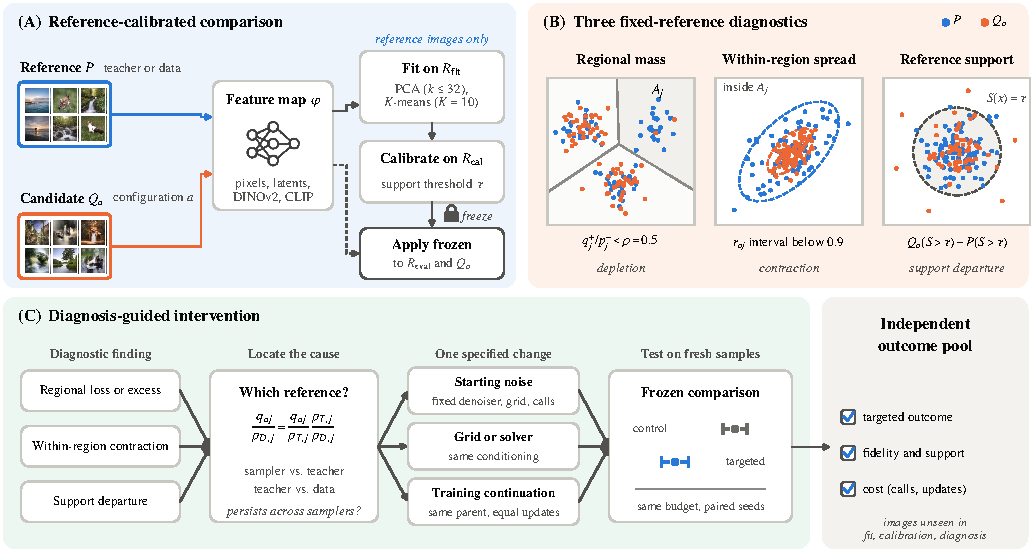
\includegraphics[width=\textwidth,pagebox=cropbox]{../figures/pipeline_overview.pdf}
\caption{Reference-calibrated diagnosis and repair.
(A) Reference and generated images use the same feature map $\phi$.
Fit regions on $R_{\rm fit}$, calibrate the support threshold on
$R_{\rm cal}$, and apply the frozen regions to the reference evaluation
pool and candidate samples. (B) The diagnostics measure regional mass,
within-region spread, and departure from reference support. In region
$j$, $p_j$ and $q_j$ are reference and candidate masses. The depletion
criterion is $q_j^+/p_j^-<0.5$ at the illustrated threshold, where $+$
and $-$ denote upper and lower confidence bounds. Contraction requires
the spread interval to lie below 0.9. (C) Compare the targeted change
with its control on independent outcomes and record fidelity and cost.
Images and point clouds are illustrative.}
\label{fig:pipeline}
\end{figure*}

\section{Introduction}
\label{sec:intro}
Two generators can have the same global variance while assigning very
different probabilities to parts of the image distribution. For a
few-step sampler, that difference determines what needs to change.
Changing the starting noise can recover image neighborhoods lost during
sampling. A digit that remains absent under several adequate samplers
calls for a test of the training distribution. The two cases require
different controls and different outcomes.

Existing occupancy tests can detect a change in a fixed region
\cite{richardson2018ndb}. To act on that change, we need to know how
large it is, what reference it is relative to, and whether an
intervention improves the target without violating fidelity criteria.
We fix the reference, regions, and effect sizes before evaluation.
A longer teacher sampler measures the change introduced by a faster
sampler. Observed data can reveal an imbalance shared by both.
Conditional spread then measures variation among samples in the same
region or under the same prompt.
\begin{figure}[t]
\centering
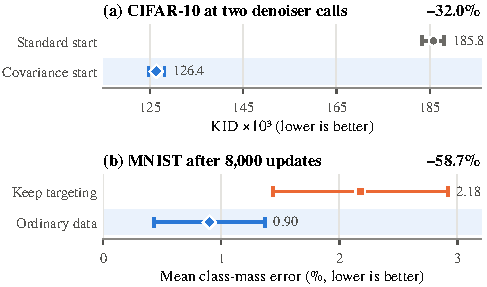
\includegraphics[width=\linewidth]{../figures/overview.pdf}
\caption{Reference-calibrated diagnosis enables independently verified repairs.
(a) Covariance initialization improves two-call CIFAR-10 Kernel Inception
Distance over five generated-sample panels from one checkpoint. (b) Ordinary
continuation reduces class-mass error in a separate equal-8,000-update
MNIST study across three training seeds. Whiskers show ordinary 95\%
Student-$t$ intervals.}
\label{fig:overview}
\end{figure}

Two confirmed repairs demonstrate this approach (Fig.~\ref{fig:overview}).
On CIFAR-10, covariance initialization reduces two-call Kernel Inception
Distance (KID) by 32.0\% and increases real-data DINO coverage from 0.206
to 0.288. Evaluating the same outputs against a separate CIFAR-10.1 reference
gives 32.7\% lower KID. On MNIST, signed regional measurements identify
overcorrection after targeted restoration. A separate equal-update
ordinary-data continuation lowers class-mass error by 58.7\% within the
declared fidelity margins.

Consider a reference with probabilities $(1/4,1/2,1/4)$ at feature
values $(-2,0,2)$ and a candidate with equal mass at $-\sqrt{2}$ and
$\sqrt{2}$. Both have mean zero and variance two. The fixed region
$[-1/2,1/2]$ contains half the reference mass and zero candidate mass.
If 100 independent draws per distribution give 50 reference hits and zero
candidate hits, the one-region audit gives a 97.5\% simultaneous upper
bound of 0.133 on the mass ratio. This certifies depletion at the
declared threshold of 0.5 (Sec.~\ref{sec:method}).

We ask three questions. Which regions lose or gain probability relative to
a fixed reference? How does variation within a region or prompt change
when fidelity is measured separately? Which controlled interventions
repair the diagnosed deficit on independent samples?

We contribute a fixed-reference audit that distinguishes regional loss,
within-region contraction, and departures from reference support. Its
finite-sample bounds show how the resolution of a regional diagnosis
depends on the effect size, reference mass, and comparison family.
We demonstrate two matched-budget repairs and explain why pooled
spread, within-prompt spread, and comparisons to different teachers
can give different answers about the same generator.

\section{Related work}
\label{sec:related}
Precision and recall, density and coverage, and authenticity quantify
different aspects of fidelity and coverage~\cite{kynkaanniemi2019improved,naeem2020density,alaa2022faithful}.
Vendi measures kernel diversity~\cite{friedman2023vendi}. Scendi separates
prompt-associated variation~\cite{ospanov2025scendi}, and Conditional
Vendi and Rényi kernel entropy distinguish prompt and model variation
and use these measurements to guide generation~\cite{jalali2026conditional}.
The number-of-statistically-different-bins test compares occupancy in
fixed $K$-means regions~\cite{richardson2018ndb}. Its equality test can
detect a change in occupancy even when the data cannot certify a
practically meaningful depletion. We specify the magnitude to certify,
then use separate measurements of conditional spread and fidelity to
design an intervention test.

Few-step interventions can change the solver, the generator, or the
conditions at sampling time. DDIM, DPM-Solver++, and UniPC change how a
fixed denoiser is integrated~\cite{song2021ddim,lu2022dpmpp,zhao2023unipc},
while consistency and distribution-matching distillation change the
learned generator~\cite{luo2024lcm,luo2023lcmlora,yin2024dmd2}.
Data-dependent priors, starting-noise corrections, and schedule design
address the match between initial noise and the sampler
\cite{lee2022priorgrad,zheng2023truncated,hu2024onemore,lin2024flawed,sabour2024align}.
Conditioning noise, early-step hybrids, covariance-aware sampling, and
adaptive computation provide other intervention points
\cite{sadat2024cads,gandikota2026diversity,schioppa2026covariance,zhang2025adadiff,li2024budgetfusion,binici2026adsc}.
Exact Gaussian solutions and spectral transfer analyses distinguish
initialization from integration error~\cite{pierret2025gaussian,benita2025spectral}.
We use this distinction to test a covariance-only change on a fixed
denoiser and time grid, and account separately for the cost of diagnosing
a deficit and generating new images.

\section{A fixed-reference audit for distribution repair}
\label{sec:method}
Figure~\ref{fig:pipeline} summarizes the audit, from a fixed reference
to a controlled intervention test.
Let $P$ be the reference law and $Q_a$ the output law of configuration $a$,
which specifies the checkpoint, schedule, guidance, solver, and randomization.
Use the law $P_T$ of a resolved teacher to measure sampler-relative change
or the observed-data law $P_D$ to measure data-relative representation.
Declare the representation, regions, effect sizes, fidelity margins, comparison
family, and budget. Disjoint reference pools $R_{\rm fit}$, $R_{\rm cal}$,
and $R_{\rm eval}$ fit the regions and support score, calibrate its threshold,
and estimate reference outcomes, respectively. Candidate evaluation images
enter neither fit nor calibration. We use a diagnosis pool to choose the
intervention and a separate outcome pool to test the frozen comparison.
The audit returns a regional decision and uncertainty interval, a
conditional spread estimate, and fidelity and cost measurements for each
tested configuration. An unresolved certificate leaves open both the
presence and the absence of a practically meaningful deficit.

Let $\mathcal X$ be the image space and $\phi:\mathcal X\to\mathbb R^d$
the representation with $d$ features. Reference-fit principal component
analysis (PCA) gives a mean $m$, an orthonormal
basis $U\in\mathbb R^{d\times k}$ with up to $k=32$ retained directions,
and coordinates $z(x)=U^\top(\phi(x)-m)$. For feature regions, fit
$K=10$ $K$-means cells after scaling each coordinate by its reference-fit
standard deviation. The fixed assignment $J(x)\in\{1,\ldots,K\}$ defines
$A_j=\{x:J(x)=j\}$. Pixel, latent, DINOv2, and CLIP features offer
different views of the images~\cite{oquab2024dinov2,radford2021clip}.
For semantic regions, apply the same classifier and rejection rule to
both laws. The partition includes rejection, and rejected images stay
in the denominator of each region's probability. Held-out real
accuracy validates the labeling rule on real images. Feature fidelity
and uncurated samples help assess its interpretation on generated images.

For image $X$ under $P$, let $Y=\phi(X)$. Write $p_j=P(X\in A_j)$ and
$q_{aj}=Q_a(X\in A_j)$. Let $\mu$ be the mean of $Y$ under $P$, and let
$\mu_j$ and $\Sigma_j$ be its mean and covariance conditional on $A_j$.
Then
\begin{equation}
\operatorname{Cov}_{P}(Y)
=\sum_j p_j\Sigma_j+\sum_j p_j(\mu_j-\mu)(\mu_j-\mu)^\top.
\label{eq:totalcov}
\end{equation}
Terms with zero mass contribute zero. The first term averages within-region covariance. The second measures
separation of regional means. Either term can change with regional mass,
which explains why pooled spread alone cannot identify a deficit.

To certify a regional change, fix all events before drawing evaluation
images independently within each law. Reference and candidate draws may
be paired across laws. The guarantee assumes fixed evaluation sizes.
Pooling samples drawn under different prompts requires a sampling model
for the prompt mixture. We report prompt-level uncertainty separately.
Let $M$ count all declared region, condition, configuration, and
representation comparisons. Let $[p_j^-,p_j^+]$ and $[q_{aj}^-,q_{aj}^+]$
be exact binomial intervals with per-tail error
$\varepsilon=\alpha_{\rm occ}/(4M)$~\cite{clopper1934confidence}, where
$\alpha_{\rm occ}$ is the family error budget. The union bound yields
intervals for $q_{aj}/p_j$ in all positive-mass regions with simultaneous coverage at least
$1-\alpha_{\rm occ}$:
\begin{equation}
\left[q_{aj}^-/p_j^+,\ q_{aj}^+/p_j^-\right].
\label{eq:occupancy}
\end{equation}
For $p_j>0$, the upper endpoint is infinite when $p_j^-=0$.
Only eligible regions receive a ratio decision. An eligible region has
$p_j^-\geq\pi_{\min}$, a minimum reference mass. An upper endpoint below
the ratio threshold $\rho$ certifies \emph{depletion}; a lower endpoint
above $\rho$ certifies \emph{retention} at that resolution. Otherwise the
test is unresolved. Defaults are $\rho=0.5$ and $\pi_{\min}=0.01$.
For signed mass balance, bound $q_{aj}-p_j$ by
$[q_{aj}^--p_j^+,q_{aj}^+-p_j^-]$. The interval must lie below, above,
or within $[-\delta,\delta]$ to certify depletion, excess, or equivalence,
respectively. The digit study uses $\delta=0.03$ and charges the shared
reference bounds once (Supp.~Sec.~C.8).

With zero observations among $n_Q$ candidate draws,
$q_{aj}^+=1-\varepsilon^{1/n_Q}$. For an eligible region and
$0<\rho p_j^-<1$, certifying depletion in \cref{eq:occupancy} requires
\begin{equation}
n_Q>\frac{\log\varepsilon}{\log(1-\rho p_j^-)}.
\label{eq:planning}
\end{equation}
Rare regions and broad comparison families therefore demand more samples.
Even zero candidate counts cannot certify depletion in an ineligible region.

To measure variation separately from mass, compare the covariance traces
of the unwhitened coordinates within $A_j$:
\begin{equation}
r_{aj}=\frac{\operatorname{tr}\operatorname{Cov}_{Q_a}[z(X)\mid A_j]}
{\operatorname{tr}\operatorname{Cov}_{P}[z(X)\mid A_j]}.
\label{eq:spread}
\end{equation}
This ratio is defined when the region has positive mass under both laws
and the reference trace is positive. The trace sums coordinate variances
after centering each law separately.
A finite estimated log-ratio interval requires at least 30 samples from
each law and positive sample trace in both. Approximate influence-function intervals
wholly below 0.9 or above 1.1 flag contraction or expansion. For text-to-image,
we divide mean within-prompt trace for the candidate by that of the reference
in each representation and bootstrap whole matched prompts.

A support score $S(x)$ combines the whitened distance to the nearest
reference-fit point and the scaled PCA residual norm in quadrature.
The residual captures departures in directions discarded by projection,
and its scale is the median fit residual, floored at $10^{-6}$.
In the notation above the score is
\begin{equation}
S(x)=\sqrt{d_{\rm NN}(x)^2+
\bigl(\|\phi(x)-m-Uz(x)\|_2/s_{\rm res}\bigr)^2},
\label{eq:support}
\end{equation}
where $d_{\rm NN}(x)$ is the nearest fit-sample distance in whitened PCA
coordinates and $s_{\rm res}$ is the residual scale (Supp.~Sec.~C.1). With $n_{\rm cal}$
exchangeable reference calibration samples, its threshold $\tau$ is
the $\lceil(n_{\rm cal}+1)0.95\rceil$-th score in ascending order
\cite{vovk2013conditional}. If this rank is unavailable, the gate is unresolved.
Independent evaluations estimate $Q_a(S>\tau)-P(S>\tau)$.
Exact binomial endpoints bound this excess tail probability (Supp.~Sec.~A.3).
The gate passes if its upper bound is at most 0.05 and fails if its lower
bound exceeds 0.05. Otherwise it is unresolved. The feature-only default
gives occupancy and support error budgets of 0.025 each. The approximate
spread intervals are outside that exact error guarantee. Signed-balance
and routing follow-ups allocate 0.025/0.0125/0.0125 to mass/fidelity/support.
CIFAR selection also checks teacher precision, text-to-image checks alignment
and learned preference, and digits use classifier consensus and feature
precision. Expansion with a failed support gate is off-reference expansion.

For the same semantic event, let $p_{D,j}=P_D(A_j)$ and $p_{T,j}=P_T(A_j)$.
When both are positive, $q_{aj}/p_{D,j}=(q_{aj}/p_{T,j})(p_{T,j}/p_{D,j})$
separates sampler--teacher from teacher--data mass differences.
Teacher-relative deficits motivate changing the starting noise with the
denoiser, grid, and call budget fixed, or changing the grid or solver under
the same conditioning. A validated data-relative imbalance that persists
across qualified samplers motivates comparing ordinary and targeted
continuations from the same parent at equal update budgets. Persistence across adequate
samplers motivates a training comparison because the tested
longer samplers did not resolve the deficit. Freeze the
comparison after diagnosis and evaluate its targeted outcome, fidelity,
coverage, and cost on independent samples. Final-sample deficits can have
several causes. These controls test the effect of one specified change.

\subsection{Validation makes the diagnostic resolution explicit}
\label{sec:supportcontrols}
Controlled deletions verify which deficits the audit resolves. Removing one
joint Gaussian component while retaining all marginal modes is detected
in 200/200 trials at 1,000 samples per set. NDB also detects every joint
removal, while both projected rules detect 0/200. Combined removal,
contraction, and translation produce all three labels in 200/200 trials.
Rotation yields support departure in 198/200 trials with no expansion.

On cached image features, removing a 4.19\%-mass region is detected in
0/200, 196/200, and 200/200 trials at 250, 1,000, and 4,000 samples per set.
The smallest Gaussian null yields 4/200 expansion flags from the
approximate spread interval (Supp.~Sec.~C).

\begin{figure}[t]
\centering
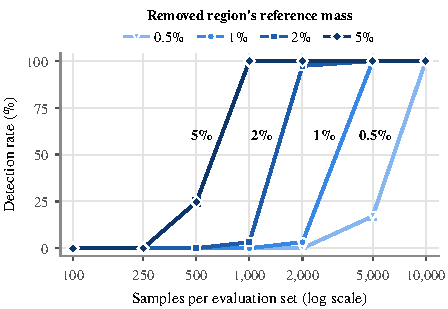
\includegraphics[width=\linewidth]{../figures/support_power_main.pdf}
\caption{Regional certificates have measurable resolution.
Complete removal, $M=10$, $\rho=0.5$, $\alpha_{\rm occ}=0.025$,
and eligibility 0.001 (distinct from the default 0.01).
Each point is 2,000 recorded trials with its saved exact 95\% binomial interval;
secondary analysis at the full-audit error level.}
\label{fig:support-main-power}
\end{figure}

Rare regions require more samples. In the power experiment with eligibility
0.001, detection for a 1\%-mass region rises
from 3.25\% at $n=2{,}000$ to 99.9\% at $n=5{,}000$
(Fig.~\ref{fig:support-main-power}); increasing the family from 10 to 440
reduces the latter to 73.95\%. With ten regions, 5,000 samples per set,
and a true ratio of 0.5, NDB flags a change in 83.4\% of trials.
The depletion test certifies a ratio below 0.5 in zero trials
(Supp.~Sec.~C.5). Equality testing can therefore flag a regional
change at sample sizes where an effect-size certificate remains unresolved.
The choice depends on whether the decision requires evidence of any change
or a lower bound on its magnitude.

\section{Controlled repairs and interpretable comparisons}
\label{sec:experiments}
Table~\ref{tab:repair-summary} summarizes the two controlled repairs.
On CIFAR-10, changing the initial covariance at a fixed denoising budget
improves agreement with real images, while a large share of generated
images still falls in a single teacher region. On MNIST, the comparison
starts from the same targeted parent and holds the update budget fixed.
Returning to ordinary training addresses the diagnosed excess and improves
mass balance across digits, with all-class equivalence unresolved.

\begin{table*}[t]
\centering
\caption{Matched-budget outcomes for the two repairs. CIFAR-10 pairs five
fresh generated panels from one checkpoint. The KID interval has nominal
95\% simultaneous coverage across five contrasts under the panel-effect
approximation. MNIST pairs three training
seeds and uses 97.5\% intervals for each of two prespecified outcomes.
Intervals condition on the fixed evaluation references. The coverage row
reports an ordinary paired 95\% interval. The largest teacher region has
reference mass 0.3535. Its row reports pooled masses.}
\label{tab:repair-summary}
\begin{tabular*}{\textwidth}{@{\extracolsep{\fill}}llrrr@{}}
\toprule
Study and matched budget & Outcome & Control & Repair & Paired difference [interval] \\
\midrule
CIFAR-10, two denoiser calls & Kernel Inception Distance $\downarrow$ &
0.1858 & 0.1264 & $-0.05938\;[-0.06138,-0.05739]$ \\
& Real-data coverage $\uparrow$ & 0.206 & 0.288 & $+0.0821\;[0.0672,0.0970]$ \\
& Largest teacher-region mass & 0.9730 & 0.9129 & \textemdash \\
\addlinespace
MNIST, 8,000 updates & Mean digit-mass error $\downarrow$ &
0.02177 & 0.00900 & $-0.01277\;[-0.01878,-0.00676]$ \\
& Digit-3 mass error $\downarrow$ & 0.06837 & 0.00747 &
$-0.06090\;[-0.11814,-0.00366]$ \\
\bottomrule
\end{tabular*}
\end{table*}

\subsection{Covariance initialization improves two-call KID and coverage}
\label{sec:cifar}
Covariance initialization lowers two-call KID by 32.0\% and raises
real-data coverage from 0.206 to 0.288 (Fig.~\ref{fig:cifar_initializer}).
KID falls from 0.1858 to 0.1264, a paired difference of
$-0.05938$ [$-0.06138,-0.05739$] with nominal 95\% simultaneous coverage across five prespecified
Student-$t$ contrasts under the panel-effect approximation. Full-moment initialization has
similar coverage (0.290) and higher KID (0.1405). DPM++ and UniPC coincide
in this two-call comparison at KID 0.2225.
KID compares distributions in Inception feature space~\cite{binkowski2018demystifying}.
DINO coverage is the fraction of real reference neighborhoods reached
by generated features~\cite{naeem2020density}.

The experiment uses a public pretrained CIFAR-10 DDPM
\cite{krizhevsky2009cifar,ho2020ddpm}. A 20,000-image DDIM100 teacher supplies
5,000/5,000/10,000 disjoint fitting/calibration/evaluation images.
The original 22-arm study used a 2,048-image pilot and 10,000 fresh images
per arm. An ablation on its paired seeds yielded KID of 0.2054 for mean
only, 0.1413 for full moments, and 0.1261 for covariance only. It motivated
the separate six-arm confirmation on five fresh paired panels of 2,000
images from the same checkpoint. Uncertainty is over generated panels and
conditions on the fixed real-data reference (Supp.~Sec.~F.3).

The repair improves agreement with real data while leaving a large
teacher-relative deficit. Nine of ten teacher-defined DINO regions
remain depleted, and conditional spread remains contracted. The largest region holds 35.35\% of teacher images, 97.30\%
of standard two-call outputs, and 91.29\% after the covariance start
(Supp.~Sec.~C.6). The fraction within the real-training 1--99\% frequency
range rises from 0.72\% to 24.7\%, compared with 97.2\% for DDIM200
(Supp.~Secs.~F.6 and G.1).

\begin{figure}[t]
\centering
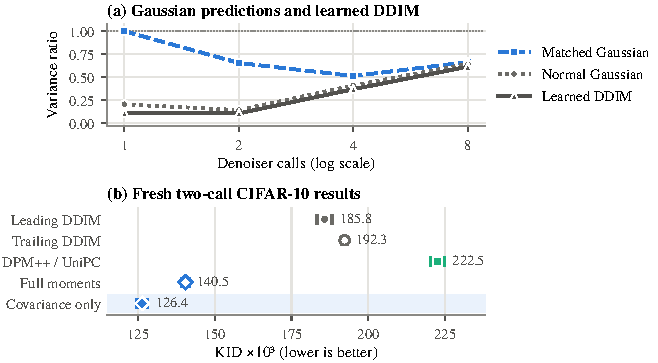
\includegraphics[width=\linewidth]{../figures/initialization_repair.pdf}
\caption{Correcting the initial covariance improves two-call generation.
(a) Saved Gaussian predictions and learned observations use a common
teacher-fit pixel basis and distinguish initialization from integration.
(b) Fresh confirmation with ordinary 95\% Student-$t$ intervals over five
generated-sample panels. DPM++ and UniPC coincide in this comparison.}
\label{fig:cifar_initializer}
\end{figure}

To explain why the starting covariance matters, consider a centered clean
Gaussian coordinate $X_0$ with variance
$\lambda>0$. Variance-preserving noising gives
$X_t=\sqrt{\bar\alpha_t}X_0+\sqrt{1-\bar\alpha_t}\,\epsilon$ at
timestep $t$, with cumulative signal coefficient $\bar\alpha_t\in[0,1]$
and independent $\epsilon\sim\mathcal N(0,1)$. Write
$v_t=\bar\alpha_t\lambda+1-\bar\alpha_t$ for the noisy variance and
$u_t=(\sqrt{\bar\alpha_t\lambda},\sqrt{1-\bar\alpha_t})$.
With the conditional mean noise predictor $\mathbb E[\epsilon\mid X_t]$
and no clipping, a deterministic DDIM
transition to an earlier timestep $s$ multiplies the coordinate by
$\sqrt{v_s/v_t}\cos\angle(u_s,u_t)$. The variance factors telescope on a
fixed grid to the clean endpoint:
\begin{equation}
\frac{\operatorname{Var}(X_{\rm out})}{\lambda}
=\underbrace{\frac{\nu_{\rm start}}{v_{\rm start}}}_{\text{initialization}}
\underbrace{\prod_{t\rightarrow s}\cos^2\angle(u_s,u_t)}_{\text{integration}},
\label{eq:gaussian}
\end{equation}
where $X_{\rm out}$ is the final coordinate, $\nu_{\rm start}$ and
$v_{\rm start}$ are actual and matched starting variances, and the product
runs over adjacent grid transitions~\cite{benita2025spectral,pierret2025gaussian}.
Matching the noisy marginal sets the first factor to one. Refining the same
endpoints improves the second factor by $\cos b\cos c\geq\cos(b+c)$
for nonnegative angles $b,c$ with $b+c\leq\pi/2$. Changing the leading-grid
budget also changes the starting timestep. The saved Gaussian predictions
give standard-normal to matched aggregate variance ratios 0.216, 0.800,
and 0.968 at two, four, and eight calls.

For a leading grid starting at timestep $t_0$, the tested initializer is
\begin{equation}
X_{\rm start}=
\big[(1-\bar\alpha_{t_0})I+\bar\alpha_{t_0}\widehat C\big]^{1/2}Z,
\qquad Z\sim\mathcal N(0,I),
\label{eq:covariance_start}
\end{equation}
where $X_{\rm start}$ is the initial noisy image, $Z$ is standard Gaussian
noise, and $I$ is the identity in 3,072-dimensional pixel space. The clean
covariance estimate $\widehat C$ uses 128 teacher-fit pixel components
and an isotropic residual. The square root is symmetric.
The two-call grid starts at $t_0=500$. The initializer changes the start
with no additional denoiser calls. Equation~\ref{eq:gaussian} extends
directionwise to shared eigenvectors. Learned trajectories at four/eight
calls correlate with the Gaussian prediction (Spearman 0.938/0.894), but
also exhibit mixing. The exact Gaussian derivation and the learned-model
checks are in Supp.~Secs.~D--F.


Evaluating the unchanged generated outputs against CIFAR-10.1v6
\cite{recht2018cifar10} lowers KID from 0.19060 to 0.12832
(32.7\%) and raises coverage from 0.3221 to 0.4268, with precision
falling from 0.9756 to 0.9580.
The paired KID difference is $-0.06228$ [$-0.06422,-0.06035$],
with 95\% simultaneous coverage across four contrasts (Supp.~Sec.~F.4).
All four prespecified KID contrasts retain their direction against this
reference, including the adverse output-map comparison below. The intervals
condition on the fixed 2,000 reference images.

\subsection{Intervention location separates spread from useful coverage}
\label{sec:numerical}
At four calls, output covariance restoration raises
pixel variance ratio from 0.376 to 0.917, while coverage falls from 0.478 to
0.332 and KID worsens from 0.0903 to 0.1024
(Fig.~\ref{fig:numerical_repair}). UniPC instead reaches coverage 0.549 and
KID 0.0694. At eight calls, output restoration again worsens KID
(0.0363 to 0.0505), while UniPC reaches 0.0245 (Supp.~Table~6).
These original frozen
comparisons retain the practical prediction transforms and clipping;
matched-grid controls hold trailing timesteps fixed, for which four-call
DDIM has KID 0.1132. Covariance-aware sampling~\cite{schioppa2026covariance}
does not improve this checkpoint within the four/eight-call ceilings when
forward and Jacobian--vector-product calls are both counted. The supplement
retains those controls and each declared cost convention.

\begin{figure}[t]
\centering
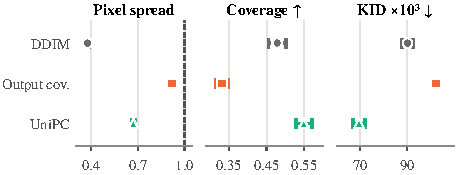
\includegraphics[width=\linewidth]{../figures/numerical_repair.pdf}
\caption{Restoring output spread can degrade useful coverage.
Four-call CIFAR-10 interventions: five paired 2,000-image panels, ordinary
95\% Student-$t$ intervals. Pixel spread is teacher-relative; coverage and KID use real data.}
\label{fig:numerical_repair}
\end{figure}

An independently pretrained variance-preserving EDM model~\cite{karras2022edm}
gives a matched-call solver comparison (Fig.~\ref{fig:edm_solver_audit}).
At 15 calls, Heun lowers KID from 0.00876 to 0.00250 while coverage falls
from 0.477 to 0.417. At 35 calls, it lowers KID from 0.00250 to 0.000413
with coverage 0.501 for both solvers. At three and seven calls, its fewer,
larger steps give worse KID. Heun uses $2K-1$ calls for $K$ integration
steps. At seven calls, Heun achieves DINO precision of 0.906, while
24.7\% of its images fall within the real-training frequency range.
This mismatch shows the value of the complementary frequency check
(Supp.~Sec.~G.1).

\begin{figure}[t]
\centering
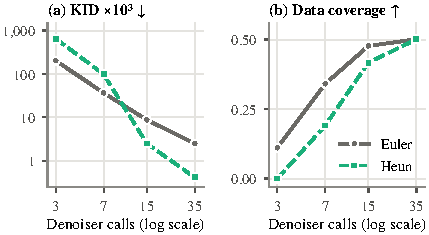
\includegraphics[width=\linewidth]{../figures/edm_solver_audit.pdf}
\caption{EDM solver choice changes with budget.
All eight arms share 2,048 noise inputs; calls and integration steps differ.
KID uses a logarithmic scale. Points are descriptive, without model-seed
uncertainty; lines connect the evaluated budgets.}
\label{fig:edm_solver_audit}
\end{figure}

\subsection{Signed mass measurements enable calibrated semantic repair}
\label{sec:mnist}
Signed regional measurements distinguish missing probability from excess
probability (Supp.~Sec.~H.2).
In MNIST~\cite{lecun1998mnist}, withholding digit~3 creates persistent
real-data-relative depletion under DDIM25, DDIM50, and DPM++25 in all three
training seeds. Two calibrated classifiers define consensus digit regions
and rejection; accepted real-image accuracy is 99.916\%, and rejection
remains in every probability denominator. The original comparison spans
three training seeds, five training states, and eleven samplers (165
evaluations); its paired restoration contrast uses the frozen
three-comparison adjustment. At DPM++25, ordinary restoration
raises digit-3 mass from 0.00087 to 0.08747, toward the data target 0.0983;
the adjusted paired increase is 0.08660 [0.07677,0.09643]. Coverage rises
from 0.727 to 0.777. Precision drops by 0.01407 versus continued withholding,
while the declared five-percentage-point fidelity margins pass against the
full-data control. Doubling the restored digit's training weight overshoots
to mass 0.1618.

To test whether ordinary training repairs the overshoot, the follow-up
compares 8,000 ordinary-data and 8,000 continued-targeting
updates from identical model, optimizer, EMA, and random states.
Each arm receives 16,000 diagnosis and 2,000 independent outcome samples.
Class-mass error averages the absolute real-to-generated probability
differences across the ten accepted digit regions.
On DPM++25 outcomes, it falls from 0.02177 to 0.00900 (58.7\%),
with paired difference $-0.01277$ [$-0.01878,-0.00676$]. Digit-3 absolute
error falls from 0.06837 to 0.00747 (89.1\%):
$-0.06090$ [$-0.11814,-0.00366$]. The two prespecified 97.5\% paired Student-$t$ intervals
use three training seeds and condition on the shared data reference.
All four fixed-reference precision and consensus fidelity constraints pass.
The ordinary continuation's classifier acceptance is 87.4\%, compared with
95.5\% on real data and 87.3\% for the full-data control.
The ordinary and targeted continuations put 9.08\% and 16.67\% of
outcome images in the digit-3 region, respectively, against 9.83\%
in the real reference. Both error reductions also hold descriptively
under DDIM25 and DDIM50 (Supp.~Sec.~H.2).
Digit-3 equivalence within $\pm0.03$ holds in all nine ordinary-continuation
seed--sampler probes; all-class equivalence and coverage superiority remain
unresolved. Diagnosis costs 48,000 images and 1.6 million denoiser calls
per checkpoint across the three probes.

The same fresh outcomes support a secondary check that includes rejection.
Each image belongs to one of ten consensus digit regions or the reject
region. We compute total variation for each branch and seed as half the
sum of the eleven absolute probability gaps to real data.
It falls from 0.1461 to 0.0854 on average, a 41.6\% reduction,
with paired difference $-0.0608$ [$-0.0828,-0.0387$] (Fig.~\ref{fig:mnist-full-balance}).
The full-distribution improvement holds in all three seeds even though
rejection remains elevated relative to real data. This secondary analysis
uses classifier events from the same paired outcomes.

\begin{figure}[t]
\centering
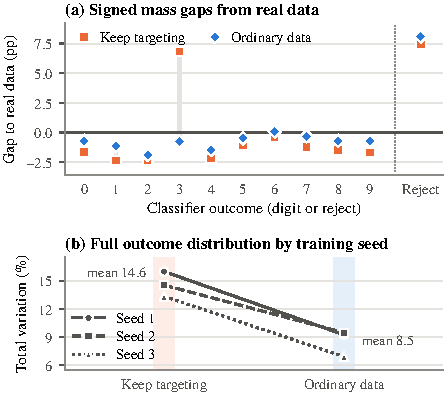
\includegraphics[width=\linewidth]{../figures/mnist_full_balance.pdf}
\caption{Ordinary continuation reduces imbalance across the complete
set of classifier outcomes. (a) Mean signed probability gaps to the
fixed real reference, in percentage points, include the reject event
(R). (b) Lines connect paired total variation estimates for the three
training seeds at the same 8,000-update budget and with 2,000 fresh
images per branch and seed. The secondary paired interval in the text
is a descriptive 95\% Student-$t$ interval.}
\label{fig:mnist-full-balance}
\end{figure}

The CIFAR-10 semantic check uses ten accepted classes plus rejection;
real-image consensus acceptance is 90.75\%, with 98.75\% accuracy among
accepted images. With one adaptation seed and 3,000 matched updates, ordinary
continuation improves DPM25 KID from 0.01479 to 0.01010 and ten-region
mean absolute mass error from 0.0247 to 0.0148. It improves both outcomes
under all five samplers and passes the declared precision/acceptance
constraints. Event-ratio weighting is worse on both metrics under all three
long-step probes. These descriptive controls show how regional measurements
and matched updates distinguish an effective continuation from a targeted
intervention whose additional benefit is unresolved.

Reference refinement supplies a further control before attributing regional
imbalance to training. The accepted frog-region mass changes from 0.138
under DPM++25 to 0.103 under DDIM200, against 0.0943 in observed data.
A separately fitted DINO classifier reproduces the direction. These fixed-event
descriptive measurements show why persistence across qualified sampler probes
is part of the training comparison: a discrepancy that shrinks with the
reference sampler is not, by itself, evidence of persistent data imbalance.

\subsection{Crossed probes separate sampler deficits from persistent depletion}
\label{sec:crossed-probes}
A short sampler can create a regional deficit that clears when
sampling is given more steps. We tested this by crossing two short samplers and three
resolved probes with five MNIST training states and three seeds
(Supp.~Secs.~H.3--H.4). Each short sampler was compared with a
25-call reference from the same checkpoint. To recommend a training
test, we also required the same real-data-relative deficit to persist
under all three resolved probes, each passing its fidelity gates.
The resulting recommendations were frozen before outcome generation.

All 12 short-sampler cases from the two withheld training states
retained digit-3 depletion under the three resolved probes and received
both recommendations. The other 18 cases received a sampler test.
An occupancy-only rule would also have flagged nine of these 18 for
training. On fresh samples, the 25-call sampler improved class-mass
error, coverage, and classifier acceptance in all 18, with a precision
loss relative to the four-call sampler. This comparison increases
inference cost from two or four calls to 25. It also leaves open
whether training could further help. Targeted checkpoints, for example,
still overrepresent digit~3, which the depletion rule does not test.

On the six cases starting from the original withheld state, combining
ordinary restoration with the resolved sampler raises digit-3 mass
to 0.08567, compared with 0.00067 for the resolved sampler with
continued withholding. Both branches use the same training update
budget. The mean class-mass error difference is $-0.00331$
[$-0.00683,0.00020$], an ordinary paired 95\% interval across three
training seeds after averaging the two short settings within each seed.
The crossed test identifies persistent depletion, while the independent
outcomes show which repair objectives improve under the chosen comparison.

\subsection{Conditioning and reference matching resolve diversity reversals}
\label{sec:t2i}
We compare SD1.5, native LCM-LoRA,
one-step DMD2, and Sana-600M
\cite{rombach2022ldm,luo2023lcmlora,yin2024dmd2,xie2025sana} on 128 held-out
PartiPrompts~\cite{yu2022parti}, with eight diagnosis and 16 separate outcome
seeds per prompt. Disjoint pools supply 32 representation-fit, 256 calibration,
and 48 development prompts. The complete matrix retains 29 SD and seven
Sana configurations. References are DDIM50 at classifier-free guidance
(CFG) 7.5 and Flow-DPM++50;
DMD2 also uses its training-matched CFG1.75 teacher. These are generator-relative
measurements; prompts supply no real-image coverage target. The evaluated
configurations include step and guidance changes, stochastic sampling,
conditioning noise, and first-base-step LCM. Native schedules and checkpoint
conversions are checked against released implementations. Prompt-level
resampling keeps each prompt's candidate/reference pairing intact and treats
its seeds as within-prompt observations.

DDIM4 has pooled DINO spread ratio 0.919 [0.910,0.928], yet within-prompt
spread ratio 1.306 [1.236,1.382] (Fig.~\ref{fig:t2i_representations}).
A secondary descriptive decomposition, specified after access to these
outcomes, explains the reversal. Within-prompt variation rises from
0.400 to 0.523 of reference pooled spread, while the between-prompt
contribution falls from 0.600 to 0.396. The larger decrease pulls the
sum below one. The within-prompt ratio uses only the reference within
component. Sampling-latent and image-re-encoding
ratios are 0.414 and 0.482. The PickScore preference proxy
\cite{kirstain2023pickapic} is 0.247 [0.227,0.268],
below the frozen 0.45 tolerance, so fidelity qualifies the interpretation
of the increased feature spread.

\begin{figure}[t]
\centering
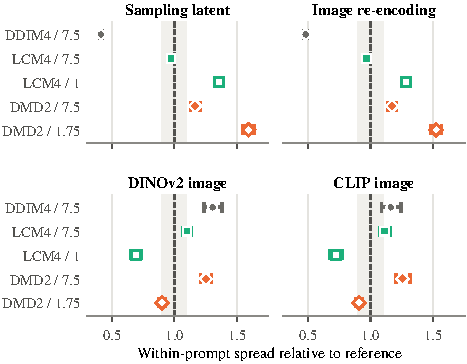
\includegraphics[width=\linewidth]{../figures/t2i_representation_reference.pdf}
\caption{Conditioning and reference matching change the measured direction.
Five comparisons, four representations: conditional trace ratios with
\emph{descriptive} 95\% paired prompt-bootstrap intervals. Rows give sampler
and teacher CFG; open markers indicate the alternate teacher. The band marks
$[0.9,1.1]$ and the dashed line marks equality. LCM CFG1 is a sensitivity;
DMD2 CFG1.75 is training-matched. The supplement retains the separate
simultaneous 20-contrast checks.}
\label{fig:t2i_representations}
\end{figure}

DMD2's DINO ratio changes from 1.251 [1.208,1.297] against CFG7.5 to
0.901 [0.873,0.929] against its matched CFG1.75 teacher. The latter is
below equality but unresolved at the 0.9 contraction margin. Against that
teacher, latent spread increases to 1.592 and learned preference reaches
0.558 [0.545,0.571]. LCM4's DINO ratio changes from 1.101 against CFG7.5
to 0.695 against CFG1; this external-guidance sensitivity is not a verified
training-matched teacher and fails CLIP support compatibility.

Sana Euler8 reduces latent spread to 0.763 [0.746,0.779] while DINO spread
rises to 1.118 [1.083,1.157]. At eight calls, Flow-DPM++ retains paired
learned preference within tolerance, 0.479 [0.471,0.487]. CADS increases
DINO spread to 1.965 [1.828,2.121] but lowers preference to
0.354 [0.339,0.369]. The same measurement discipline distinguishes added
variation from a fidelity-qualified improvement across these model families.

\subsection{What the audit establishes about choosing a sampler}
\label{sec:policy}
The original CIFAR selection rule averages KID 0.0790 across two, four,
and eight calls, compared with 0.1039 for leading DDIM and 0.0784 for
both Vendi and teacher-feature Fr\'echet selection. It chose full-moment
initialization at two calls. The later centered-covariance result tests
the intervention itself on fresh samples.

In text-to-image generation, a frozen rule screens two fast samplers
and uses a longer fallback when neither meets the diagnosis thresholds.
Its independent outcomes pass the declared fidelity and spread gates,
as do quality plus Vendi and fixed Sana DPM++8. At the same inference
cost, permuting the audit's choices across prompts leaves the coverage
and learned preference differences unresolved in both families.
The audit uses 14.06 and 14.28 denoising calls per image for Stable
Diffusion and Sana, plus 528 diagnosis calls per prompt and 38,400
reusable reference calls per family. The Sana audit also scores below
the 20-call fallback on ImageReward by 0.0261, with adjusted interval
[$-0.0461,-0.0093$]. These controls locate the operating point and the
cost of diagnosis. The full thresholds, policy table, and call-only
amortization are in Supp.~Secs.~J--L.

\section{Discussion and conclusion}
\label{sec:discussion}
A distribution repair needs a target that survives changes in how
samples are pooled and compared. Fixing the reference and a meaningful
effect size makes regional probability loss testable. Conditional spread
and fidelity then show whether changes in variation serve that target.
The crossed probes illustrate the distinction: longer sampling improves
some short-sampler deficits, while the missing digit persists across
adequate samplers when training withholds it.

The two controlled tests establish partial repairs at matched budgets.
Starting-covariance matching improves two-call agreement with real data
on one pretrained model, even though most teacher-defined regions remain
depleted. Ordinary continuation improves the full distribution of digit
classifier outcomes across three paired seeds, including rejection in
the measure. Its rejection rate still exceeds that of real data. A second
pretrained checkpoint would test transfer of the initialization result,
and independent labels for generated digits would test whether the
classifier findings track human judgments. The matched-cost prompt
shuffle leaves the advantage of per-prompt selection unresolved.

\label{audit:lastbodypage}
\clearpage
\section*{LLM Usage Statement}
OpenAI ChatGPT assisted with manuscript editing, clarity, and figure planning.
BioRender assisted with diagram formatting and icon creation.
OpenAI Codex assisted with manuscript and caption revisions, the illustrative
toy example, notation and numerical checks, LaTeX preparation, internal
critical review, plotting, table generation, and preparation of the supplied
pipeline diagram. Codex also assisted with the revised abstract, introduction, related work,
methods, and results synthesis, including a table assembled from existing
measurements, and provided internal draft assessments. Codex also generated the
classifier-event balance plot and computed its secondary paired summary
from saved outcomes. An earlier project record contains an AI-generated manuscript review whose
tool is unrecorded. The authors are responsible for the scientific claims.

{\small
\bibliographystyle{ieeenat_fullname}
\bibliography{references}}
\end{document}
